\documentclass[12pt]{article}
\usepackage{array}
\usepackage{float}
\usepackage{caption}
\usepackage{enumitem}
\usepackage{subcaption}
\usepackage[table]{xcolor} 
\usepackage{graphicx}
\usepackage{longtable}
\usepackage{ltxtable}
\usepackage{tabularx}
\begin{document}
	\noindent
	\textbf{Team:}
   	 \begin{itemize}[leftmargin=0.0cm,labelsep=0.2cm]
   	 	\item[] Badam-Osor Khaltar (badamosor)
   	 	\item[] Paul McCumber (paulmccumber)
   	 	\item[] Luke Meszar (lukemeszar)
   	 \end{itemize}
    \noindent
    \textbf{Title:} Music Playlist Manger
	\section{Summary}
	Sharing playlists of music between a large group of people can be difficult when
	everyone doesn't listen to music through the same service. This will allow people to create
	playlists in a generic format that can then be integrated into the user’s service of choice. This allows people to share their playlists with their friends who can then export it into the streaming service of their choice. 
	\section{Project Requirements}
	\rowcolors{2}{blue!10}{white}
	\begin{table}[H]
		\centering
		\label{tab:ur}
		\caption*{User Requirements}
		\begin{tabularx}{450pt}{lXl}
			ID & Description & Priority\\\hline
			UR-01 & Users can create account & High \\
			UR-02 & Users can create a playlist & High \\
			UR-03 & Users can search database for song title, album title,
			artist, and playlist name & High \\
			UR-04 & Users can add content (songs, from albums or artists) to a playlist & High \\
			UR-05 & Users can remove songs from a playlist & Medium \\
			UR-06 & Users can make playlists collaborative & Low \\
			UR-07 & Users can share a playlist & High \\
			UR-08 & Users can register their Spotify account to our service & High \\
			UR-09 & Users can register their Tidal account to our service & High \\
			UR-10 & Users can register their Google Play Music account to our service & High \\
			UR-11 & Users can export playlists into Spotify & High \\
			UR-12 & Users can export playlists into Tidal & High \\
			UR-13 & Users can export playlists into Google Play Music & High \\
		\end{tabularx}
	\end{table}
	\begin{table}[H]
		\centering
		\label{tab:nfr}
		\caption*{Non-Functional Requirements}
		\begin{tabularx}{450pt}{lXl}
			ID & Description & Priority\\\hline
			NFR-01 & Search has to be less than 20ms & High \\
			NFR-02 & Service should support thousands of concurrent users & High \\
			NFR-03 & Should be able to expand to other music services easily & Medium \\
		\end{tabularx}
	\end{table}
	\LTXtable{450pt}{functionalTable}
	\section{Use Cases}
	\begin{figure}[H]
		\centering
		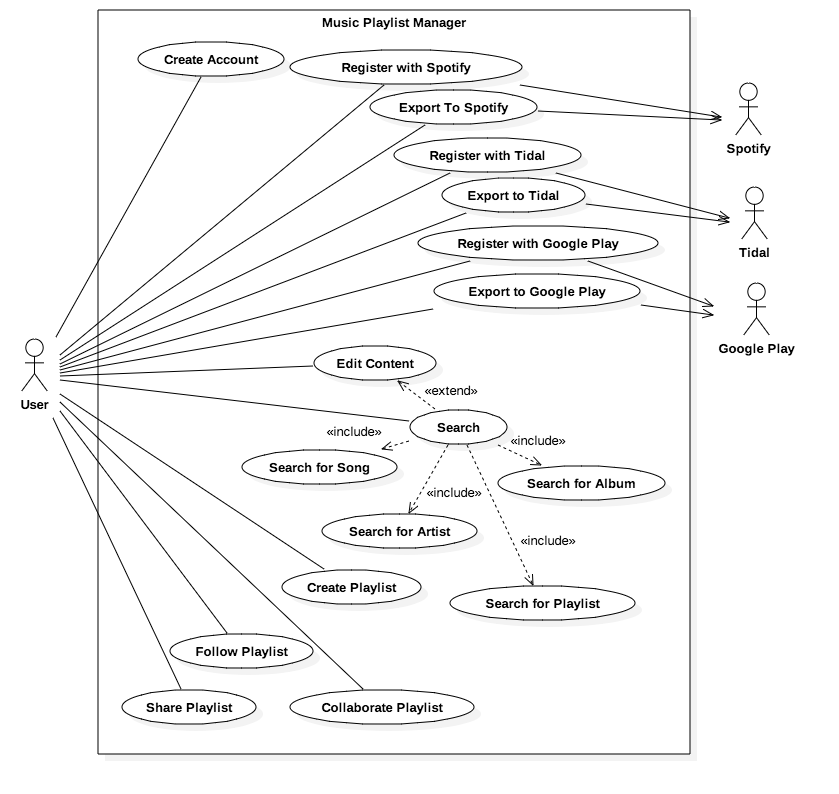
\includegraphics[scale=0.4]{SystemUseCase}
		\caption{System Use Case Diagram}
		\label{fig:sucd}
	\end{figure}
	Below are the two use case documents:
	
		\begin{center}
		\begin{tabularx}{450pt}{|r|X|}
			\hline
			\textbf{Use Case ID:} & UR-03 \\\hline
			\textbf{Use Case Name:} & Search \\\hline
			\textbf{Description:} & Users can search songs, albums, artists and playlists from database \\\hline
			&\\ \hline
			\textbf{Actors:}& Users\\\hline
			\textbf{Pre-conditions} & User is logged in \\\hline
			\textbf{Post-conditions} & User got a search result \\\hline
			\textbf{Frequency of Use:} & Daily \\\hline
			\textbf{Flow of Events:} & {\begin{tabularx}{325pt}{|c|X|X|}
					&\textbf{Actor Action}&\textbf{System Response}\\\hline
					1 & User enters a string in the search field &  \\\hline
					2 & & System find songs in database that match the string \\\hline
					3 & & System find artists in database that match the string \\\hline
					4 & & System find albums in database that match the string \\\hline
					5 & & System find playlists in database that match the string \\\hline
					6 & & System displays results \\\hline\
					7 & User views results &  \\\hline
			\end{tabularx}}\\\hline
			\textbf{Variations:} & \\\hline
			\textbf{Exceptions:} &  \\\hline
			\textbf{Developer Notes:} & \\\hline
		\end{tabularx}
	\end{center}

	\begin{center}
		\begin{tabularx}{450pt}{|r|X|}
			\hline
			\textbf{Use Case ID:} & UR-03 \\\hline
			\textbf{Use Case Name:} & Search \\\hline
			\textbf{Description:} & Users can search songs, albums, artists and playlists from database \\\hline
			&\\ \hline
			\textbf{Actors:}& Users\\\hline
			\textbf{Pre-conditions} & User is logged in \\\hline
			\textbf{Post-conditions} & User got a search result \\\hline
			\textbf{Frequency of Use:} & Daily \\\hline
			\textbf{Flow of Events:} & {\begin{tabularx}{325pt}{|c|X|X|}
					&\textbf{Actor Action}&\textbf{System Response}\\\hline
					1 & User enters a string in the search field &  \\\hline
					2 & & System find songs in database that match the string \\\hline
					3 & & System find artists in database that match the string \\\hline
					4 & & System find albums in database that match the string \\\hline
					5 & & System find playlists in database that match the string \\\hline
					6 & & System displays results \\\hline\
					7 & User views results &  \\\hline
			\end{tabularx}}\\\hline
			\textbf{Variations:} & \\\hline
			\textbf{Exceptions:} &  \\\hline
			\textbf{Developer Notes:} & \\\hline
		\end{tabularx}
	\end{center}
	
	\begin{center}
		\begin{tabularx}{450pt}{|r|X|}
			\hline
			\textbf{Use Case ID:} & UR-04 \\\hline
			\textbf{Use Case Name:} & Add Playlist Content \\\hline
			\textbf{Description:} & Users can add content to a playlist. \\\hline
			&\\ \hline
			\textbf{Actors:}& Users\\\hline
			\textbf{Pre-conditions} & Users are logged in.
			
			Users have searched for content in the system (see UR-03)
			 \\\hline
			\textbf{Post-conditions} & User has added a song or album to the playlist \\\hline
			\textbf{Frequency of Use:} & As frequently as desired \\\hline
			\textbf{Flow of Events:} & {\begin{tabularx}{325pt}{|c|X|X|}
					&\textbf{Actor Action}&\textbf{System Response}\\\hline
					1 & User selects the search term results for a song. & System displays available playlists. \\\hline
					2 & User selects playlist to add song. & System displays playlist with new song added. \\\hline
			\end{tabularx}}\\\hline
			\textbf{Variations:} & \begin{enumerate}[label=(\alph*)]
				\item 	{\begin{tabularx}{296pt}{|c|X|X|}\hline
						1 & User selects the search term results for an album. & System displays all songs from album. \\\hline
						3 & User can either add entire album or choose a song (see previous variation) & System prompts user for which playlist to add content to. \\\hline
						4 & User chooses playlist. & System displays playlist with new content added. \\\hline
				\end{tabularx}} 
				\item 
				{\begin{tabularx}{296pt}{|c|X|X|}\hline
						1 & User selects the search term results for an artist. & System displays artists albums. \\\hline
						2 & & System displays artists songs.\\\hline
						3 & User selects playlist to add song or album to (see previous two variations) & System prompts user for which playlist to add content to. \\\hline
						4 & User chooses playlist. & System displays playlist with new content added. \\\hline
				\end{tabularx}} 
			\end{enumerate}\\\hline
			\textbf{Exceptions:} &  \\\hline
			\textbf{Developer Notes:} & \\\hline
		\end{tabularx}
	\end{center}
	\section{Activity Diagrams}
		\begin{figure}[H]
		\centering
		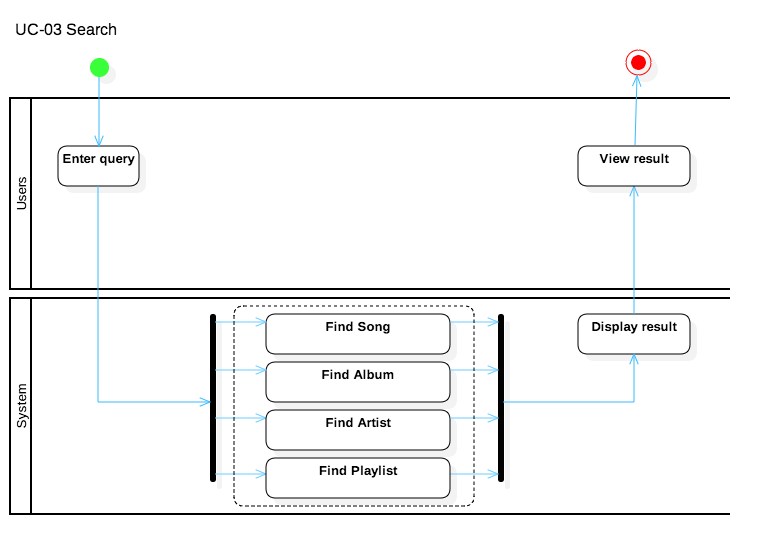
\includegraphics[scale=0.3]{SearchActivityDiagram}
		\caption{Activity Diagram for Searching}
		\label{fig:act1}
	\end{figure}
	\begin{figure}[H]
		\centering
		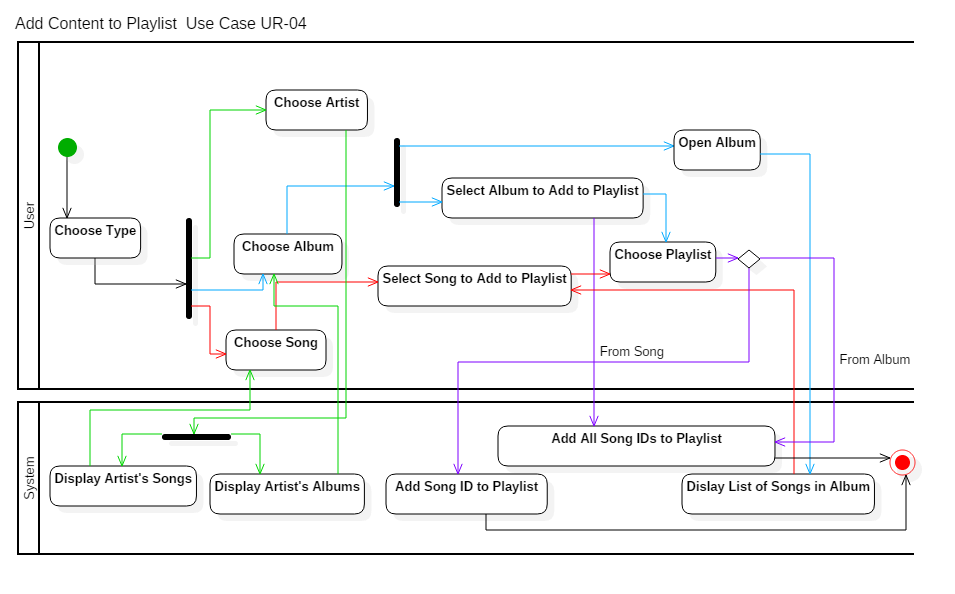
\includegraphics[scale=0.3]{ActivityDiagramAddContent}
		\caption{Activity Diagram for Adding Content}
		\label{fig:act2}
	\end{figure}

	\section{UI Mockups}
	We begin with a statechart diagram of the UI and then a closer look at all the screens for more detail. 
		\begin{figure}[H]
		\centering
		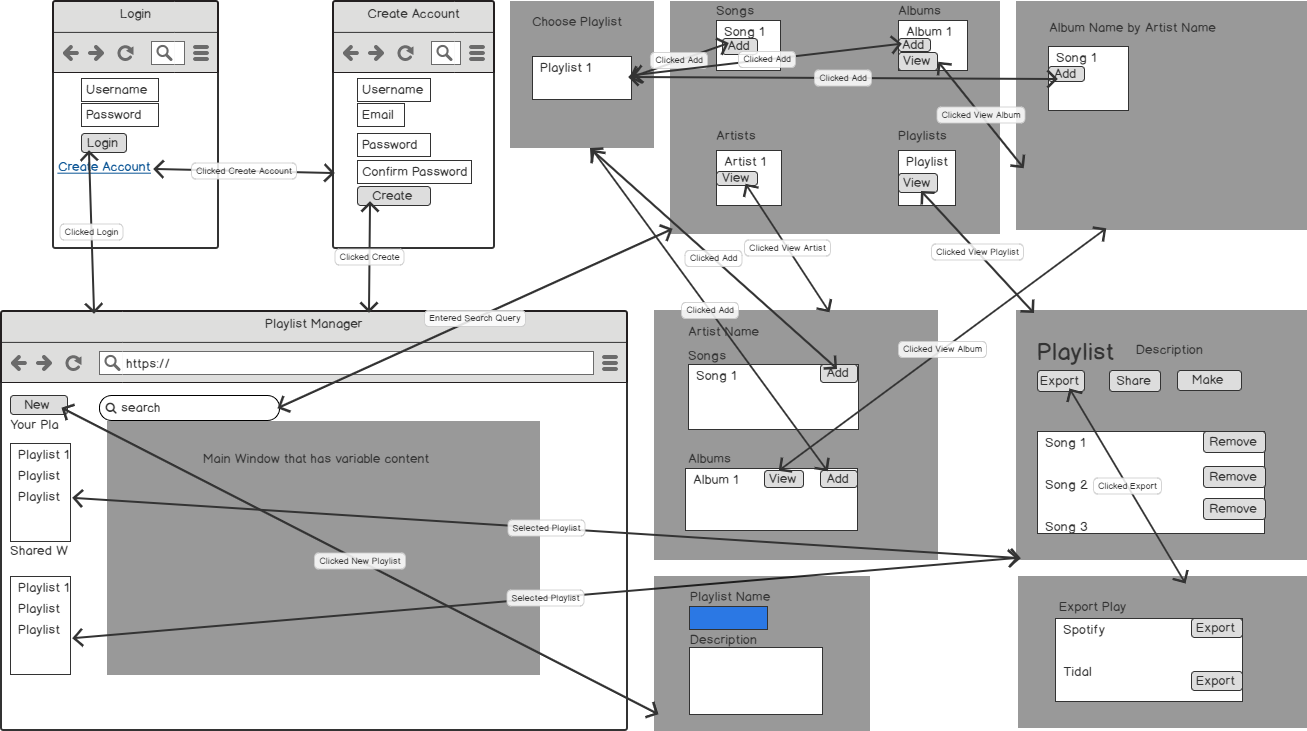
\includegraphics[scale=0.3]{StatechartDiagram.png}
		\caption{Main Window}
		\label{fig:statechart}
	\end{figure}
	\begin{figure}[H]
		\centering
		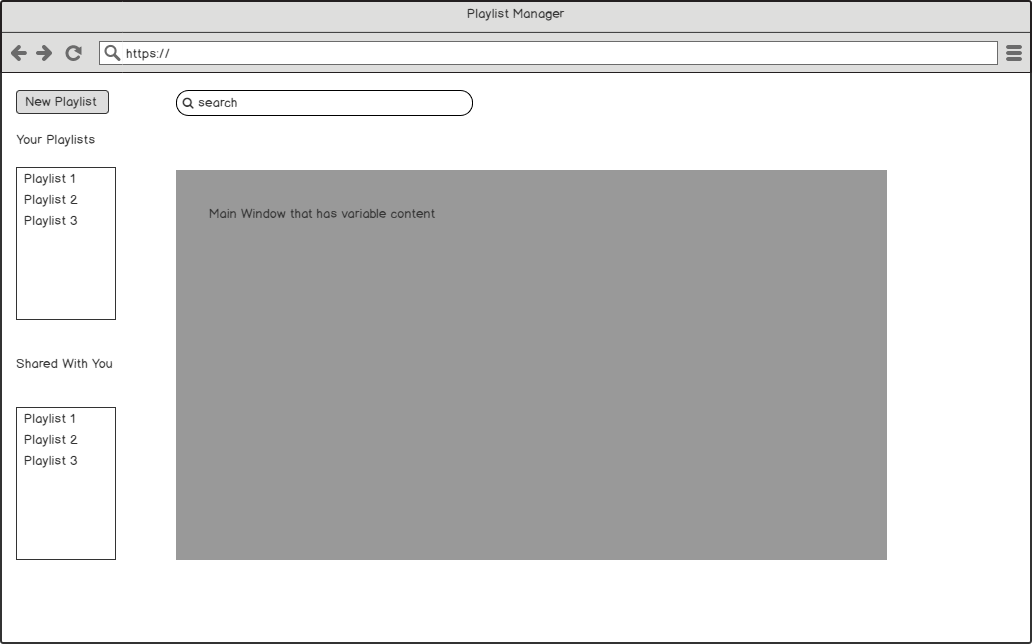
\includegraphics[scale=0.4]{GenericMainWindow}
		\caption{Main Window}
		\label{fig:gmw}
	\end{figure}
	\begin{figure}[H]
		\centering
		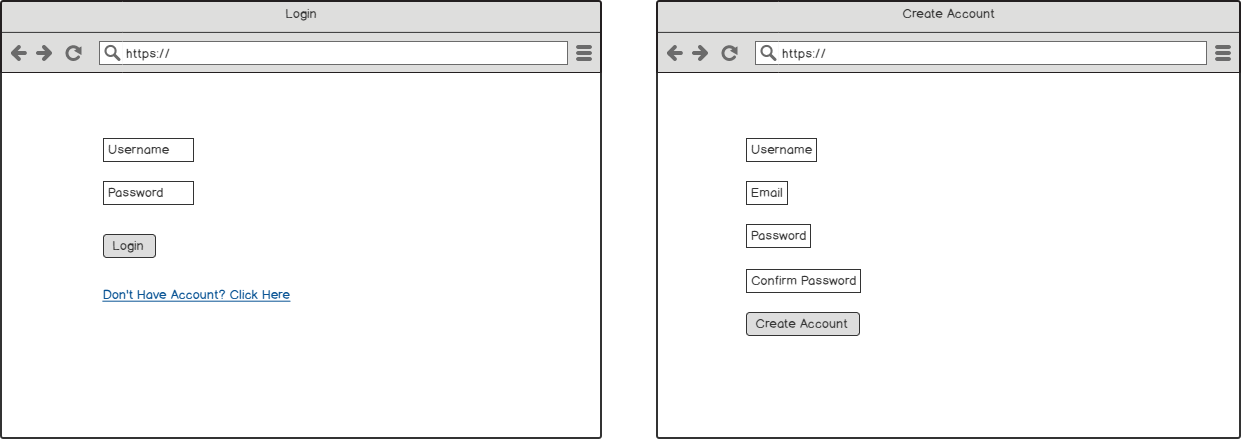
\includegraphics[scale=0.35]{CreateAccount.png}
		\caption{Login and Create Account Windows}
		\label{fig:login}
	\end{figure}
	\begin{figure}[H]
	\centering
	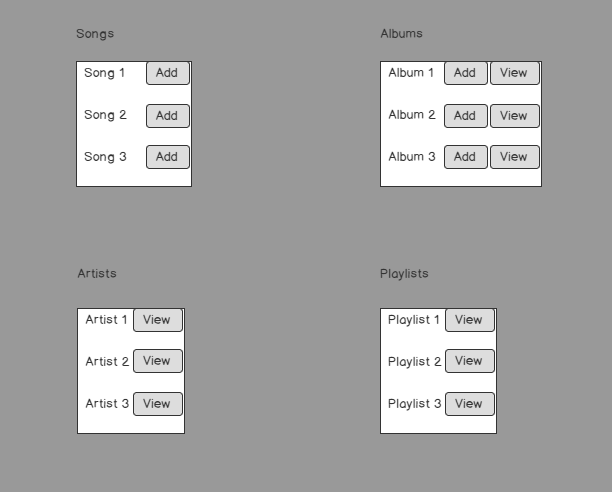
\includegraphics[scale=0.35]{SearchWindow.png}
	\caption{Search Window}
	\label{fig:search}
	\end{figure}
		\begin{figure}[H]
		\centering
		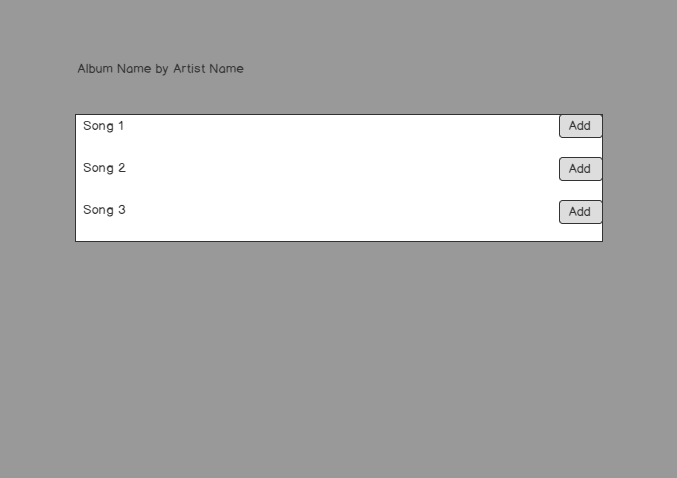
\includegraphics[scale=0.35]{AlbumWindow.png}
		\caption{Album View Window}
		\label{fig:album}
	\end{figure}
	\begin{figure}[H]
	\centering
	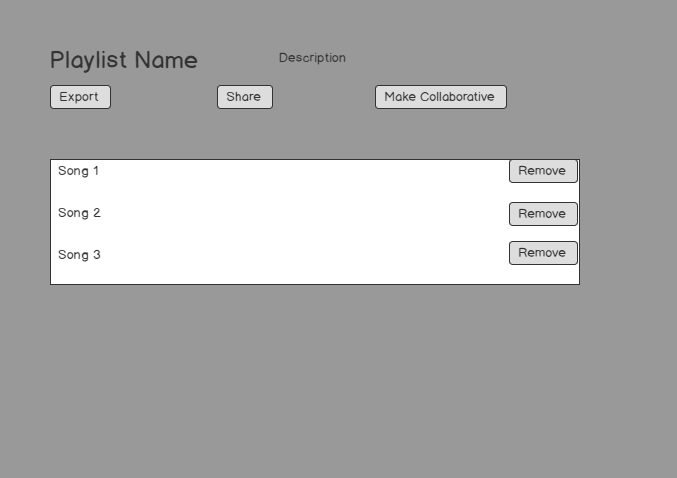
\includegraphics[scale=0.35]{PlaylistWindow.png}
	\caption{Playlist View Window}
	\label{fig:playlist}
	\end{figure}
	\begin{figure}[H]
		\centering
		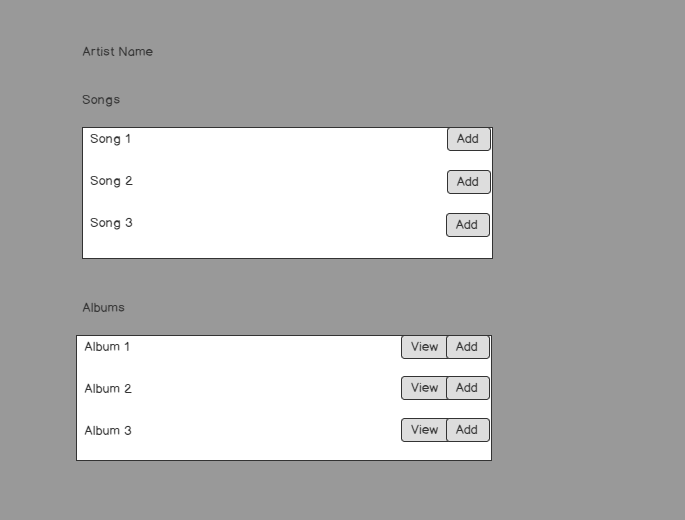
\includegraphics[scale=0.35]{ArtistWindow.png}
		\caption{Artist View Window}
		\label{fig:artist}
	\end{figure}
	\begin{figure*}[t!]
		\centering
		\begin{subfigure}[t]{0.3\textwidth}
			\centering
			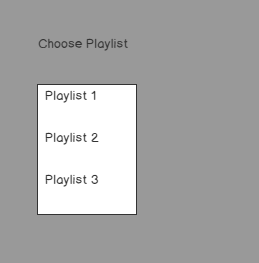
\includegraphics[scale=0.4]{ChoosePlaylistDialog}
			\caption{Choose Playlist}
		\end{subfigure}%
		~ 
		\begin{subfigure}[t]{0.3\textwidth}
			\centering
			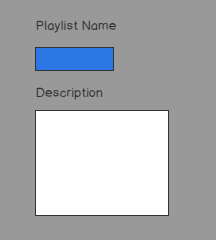
\includegraphics[scale=0.4]{NewPlaylistDialog.png}
			\caption{New Playlist}
		\end{subfigure}
		~
		\begin{subfigure}[t]{0.3\textwidth}
			\centering
			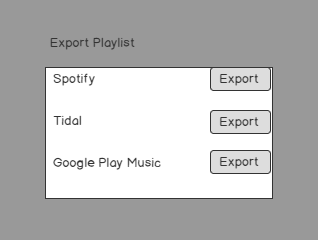
\includegraphics[scale=0.4]{ExportPlaylist.png}
			\caption{Export Playlist}
		\end{subfigure}
		\caption{Dialogs}
	\end{figure*}

	\section{Sequence Diagrams}
	\begin{figure}[H]
		\centering
		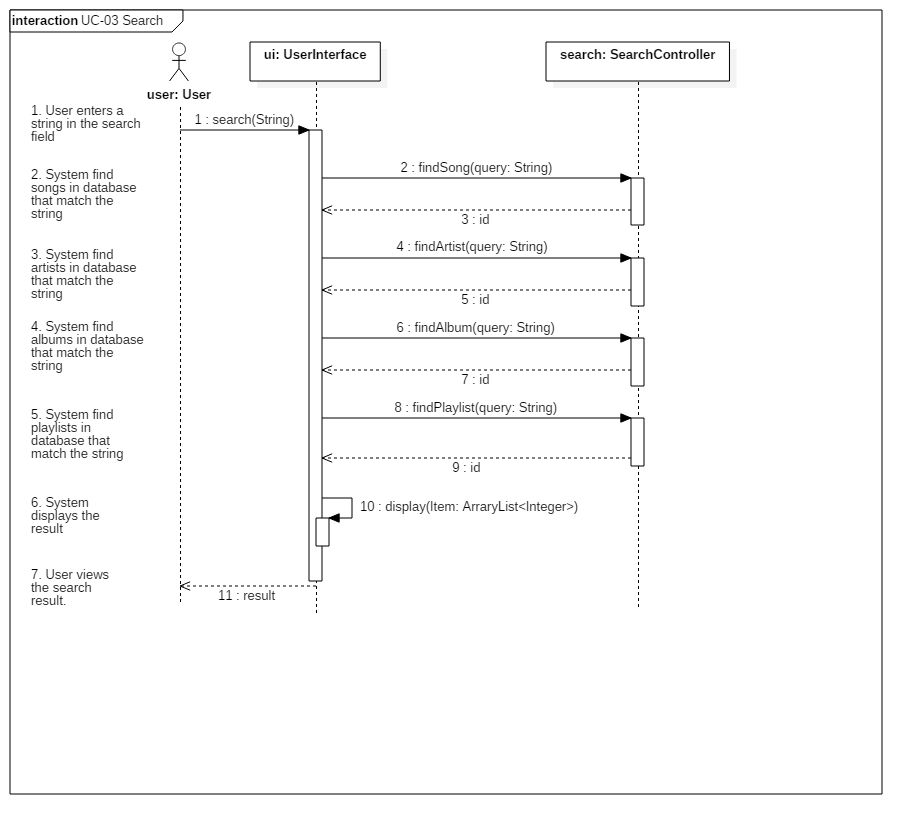
\includegraphics[scale=0.35]{UR-03Search.png}
		\caption{Sequence diagram searching}
		\label{fig:sequenceSearcj}
	\end{figure}
	\begin{figure}[H]
		\centering
		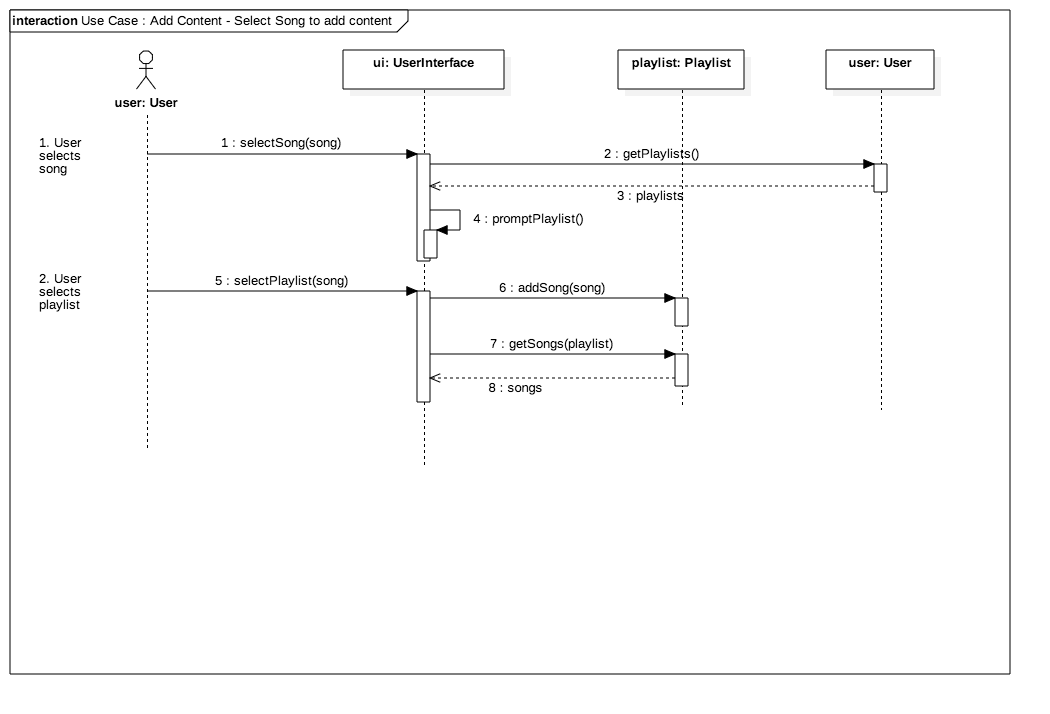
\includegraphics[scale=0.35]{UseCaseAddSong.png}
		\caption{Sequence diagram for adding a song to a playlist}
		\label{fig:sequenceSong}
	\end{figure}
	\begin{figure}[H]
		\centering
		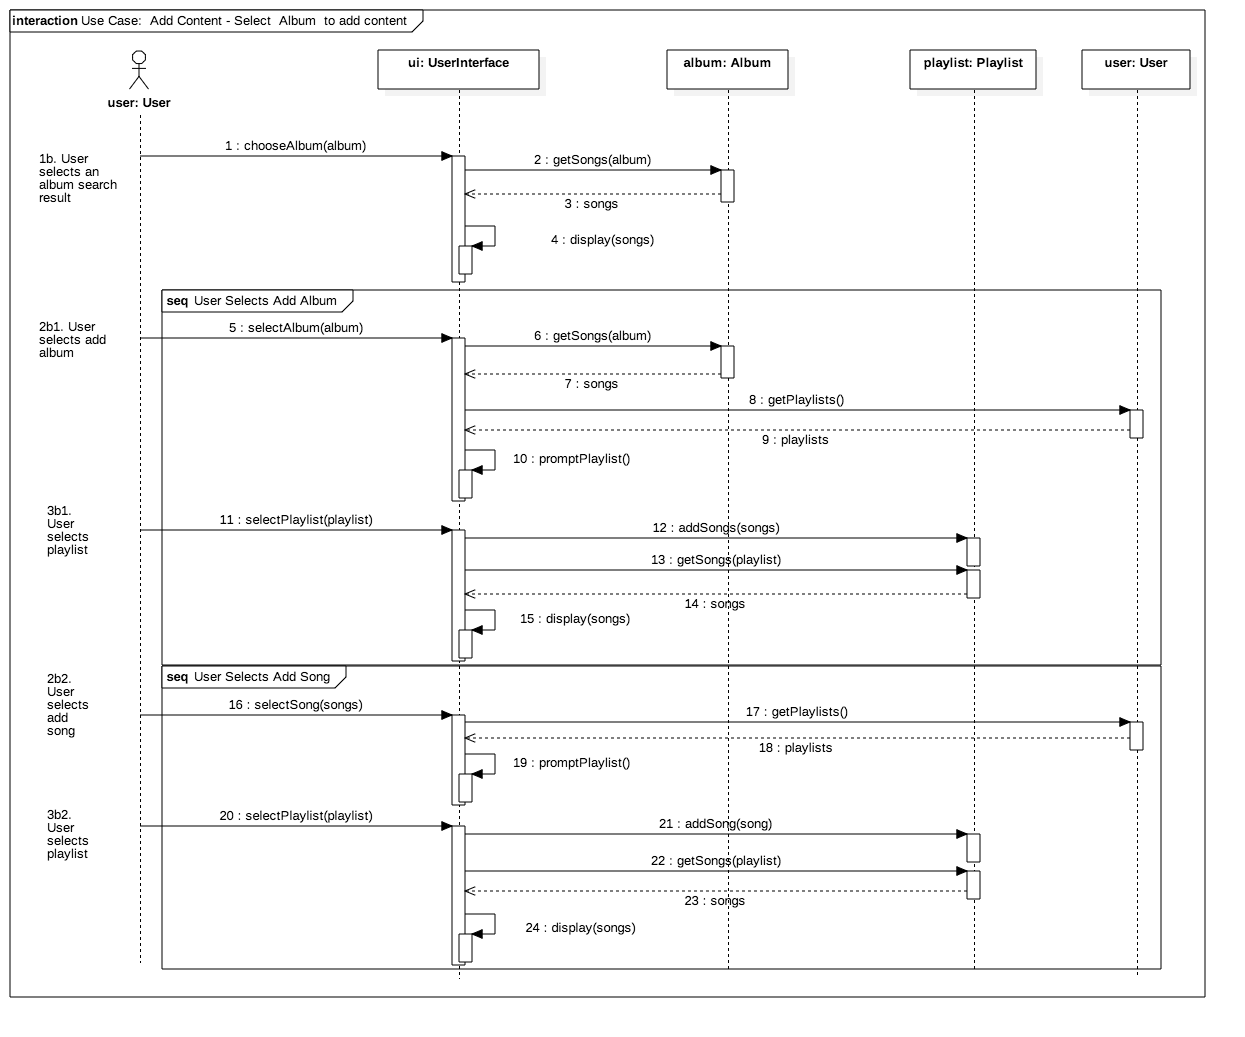
\includegraphics[scale=0.35]{UseCaseAddAlbum.png}
		\caption{Sequence diagram for adding an album's content to a playlist}
		\label{fig:sequenceAlbum}
	\end{figure}
	\begin{figure}[H]
		\centering
		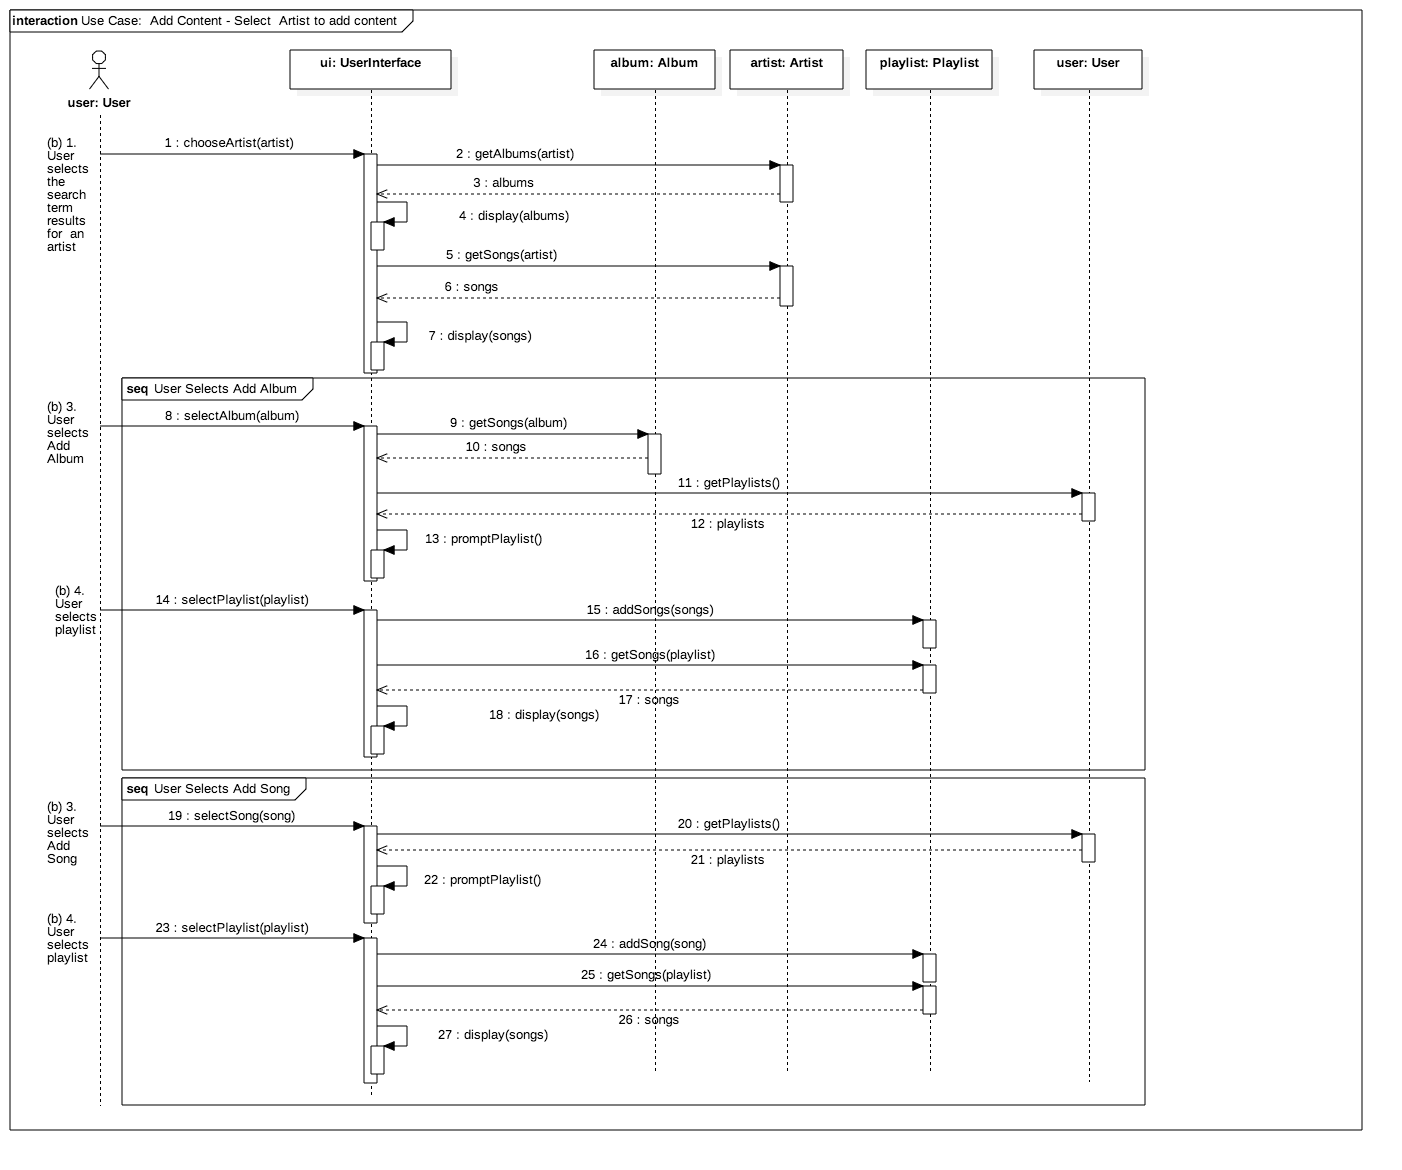
\includegraphics[scale=0.35]{UseCaseAddArtist.png}
		\caption{Sequence diagram for adding an artist's content to a playlist}
		\label{fig:sequenceArtist}
	\end{figure}
	\section{Class Diagram}
	\begin{figure}[H]
		\centering
		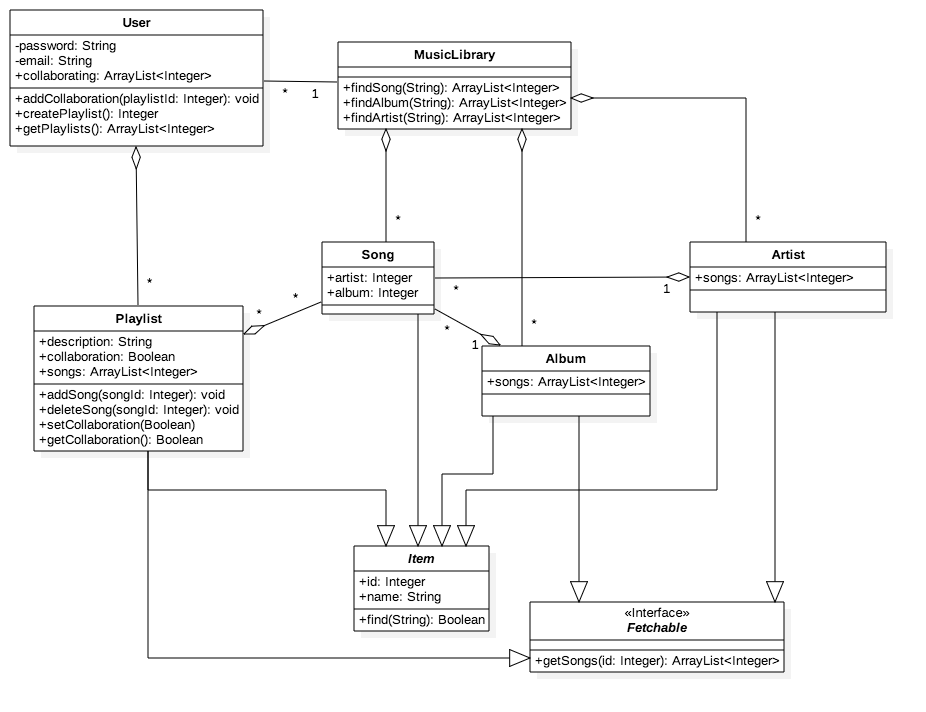
\includegraphics[scale=0.35]{MusicManagerClassDiagram.png}
		\caption{Class Diagram}
		\label{fig:classDiag}
	\end{figure}
	
\end{document}